\begin{figure*}[htbp]
    \centering
    \begin{tabular}{m{0.45\linewidth} m{0.45\linewidth} m{0.1\linewidth}}
        \begin{minipage}[b]{\linewidth}
            \centering
            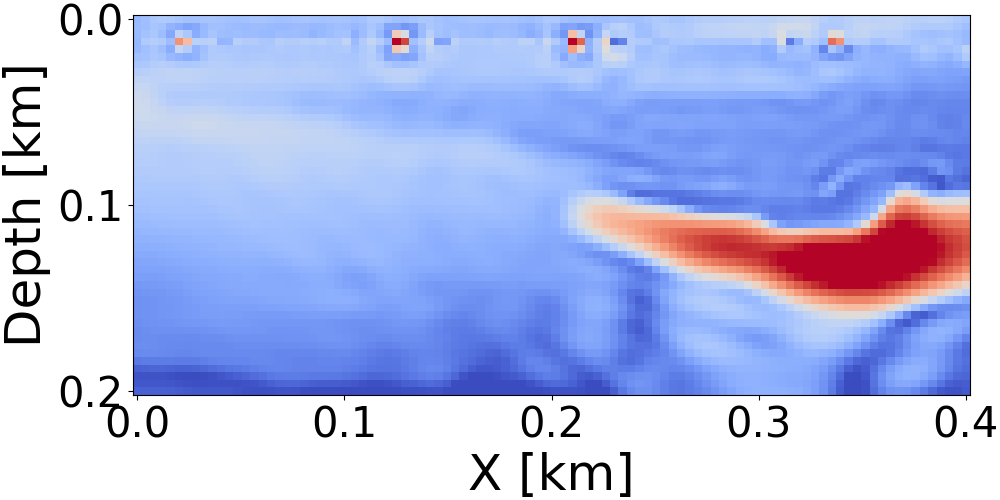
\includegraphics[width=\linewidth]{public/gradient}
            \caption*{\raisebox{2mm}{The Standard FWI Method}}
        \end{minipage} &
        \begin{minipage}[b]{\linewidth}
            \centering
            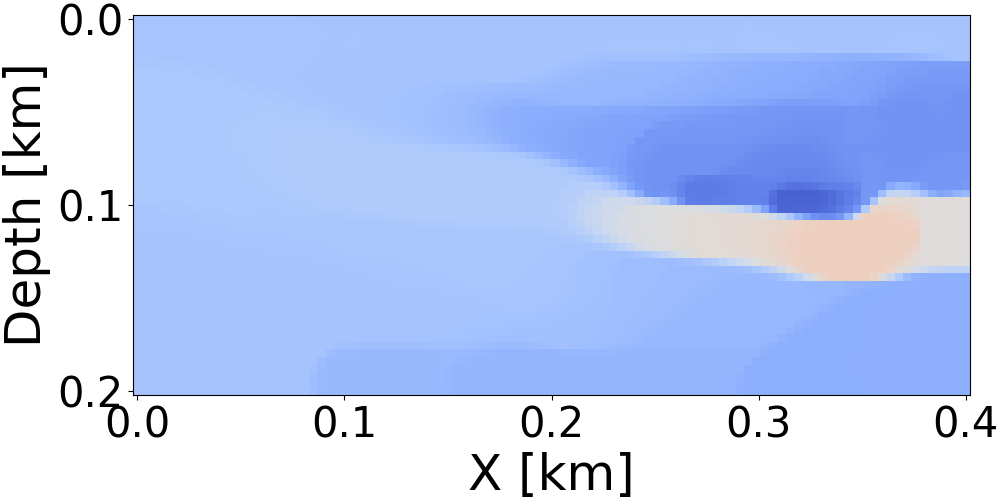
\includegraphics[width=\linewidth]{public/alpha_150}
            \caption*{Proposed Method, $\alpha = 150$}
        \end{minipage} &
        \multirow[t]{3}{*}{\raisebox{-51mm}{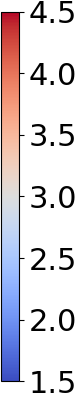
\includegraphics[height=50mm]{public/color-bar}}} \\

        \begin{minipage}[b]{\linewidth}
            \centering
            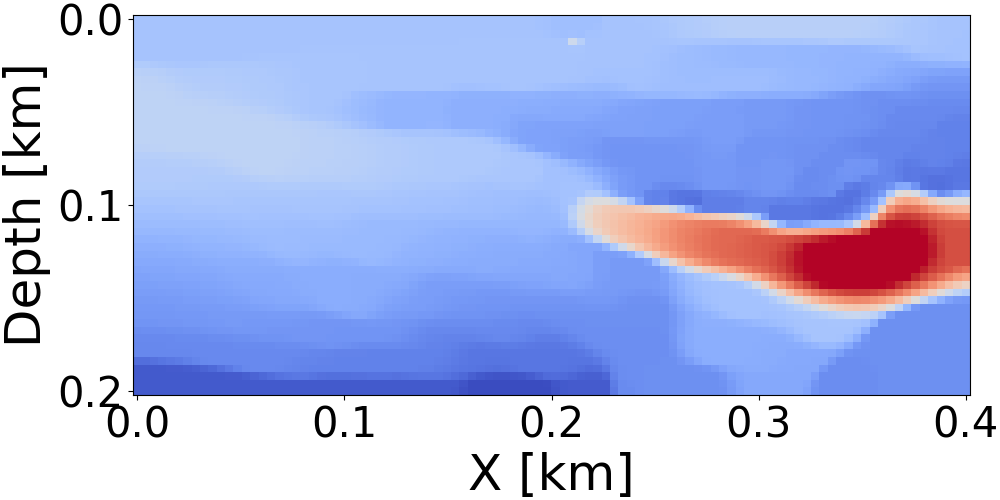
\includegraphics[width=\linewidth]{public/alpha_350}
            \caption*{Proposed Method, $\alpha = 350$}
        \end{minipage} &
        \begin{minipage}[b]{\linewidth}
            \centering
            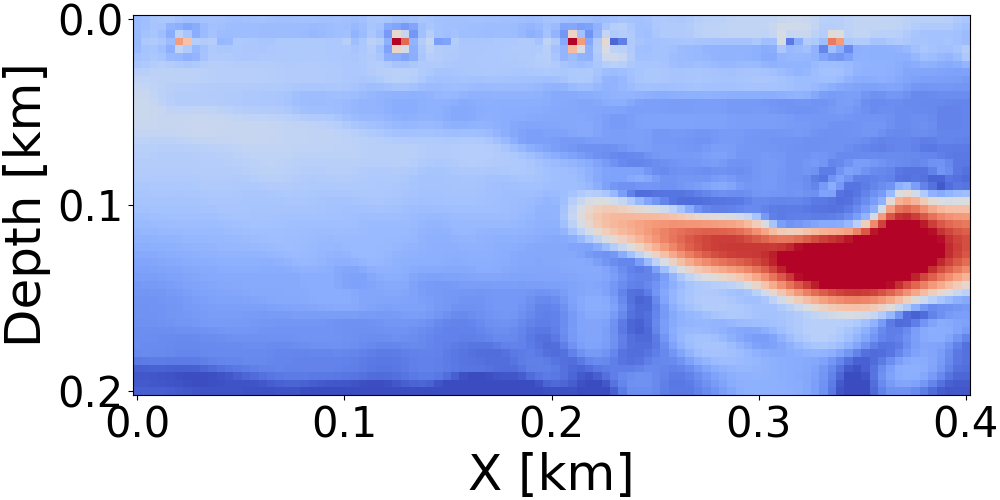
\includegraphics[width=\linewidth]{public/alpha_550}
            \caption*{Proposed Method, $\alpha = 550$}
        \end{minipage} &
    \end{tabular}
    \caption{Velocity models [km/s] and their corresponding reconstructions.}
    \label{fig:velocity-models-pure}
\end{figure*}
